%!TEX root = ../paper.tex

\section{Evaluation \& Bewertung}

Zur Bewertung der Qualität werden die Algorithmen auf verschiedensten Testdaten angewandt und die Ergebnisse anschließend ausgewertet.

Basis der Evaluation bildet einer der beiden zur Verfügung gestellten Testdatensätze. Dieser enthält eine nahezu vollständige Erfassung der Lastgänge für ein ganzes Jahr mit lediglich zwei fehlenden Einträgen. Da das Ziel der Algorithmen die Nachbildung fehlender Werte ist, werden mithilfe eines entwickelten Evaluationstools zur Evaluation Werte aus dem vollständigen Datensatz entfernt. Dies geschieht in verschiedenen Auflösungsstufen, die unterschiedlich lange Ausfallphasen simulieren. Die größte Phase ist eine ganze Woche, weiterhin wird das Entfernen ganzer Tage oder Stunden vom Tool unterstützt. Die feinste Einheit sind lediglich einzelne fehlende Elemente. Das Tool bietet für jede der Stufen einen Konfigurationsparameter an. Dieser legt den Anteil der zu entfernenden Elemente im Wertebereich von Null bis Eins fest. So werden bei einem Eingabewert von 0,5 ca. 50\% der Einträge entfernt. Die Entfernung der Werte findet dabei zufällig statt, während mit entsprechenden Intervallfenstern über die Werte iteriert wird. Zuerst werden ganze Wochen entfernt, anschließend in absteigender Reihenfolge Bereiche mit den anderen unterstützten Fenstergrößen.

Nachdem Werte entfernt und anschließend mithilfe der Algorithmen wieder interpoliert wurden, werden die Differenzen zwischen dem realen, aus dem vollständigen Originaldatensatz bekannten Datensatz und den interpolierten Werten berechnet. Die Differenzen aller einzelnen Zeitpunkte werden als euklidische Distanz zusammengefasst und bilden damit eine numerische Bewertung der Algorithmen.

Die meisten Algorithmen erfordern wie jeweils beschrieben die Definition von Konfigurationsparametern wie beispielsweise der Anzahl an Nachbarn, die in die Berechnung des Ergebnisses einfließen. Hierfür wurden jeweils die nach Meinung der Entwickler plausibelsten Werte gewählt. Aufgrund von mangelndem Expertenwissen sind diese Werte nicht zwingend optimal gewählt. Der Datenbankansatz wurde lediglich mit dem vollständigen Datensatz als Basis konfiguriert, was die Aussagekraft im Gegensatz zu einer sehr umfangreichen Sammlung verschiedener Datensätze verringert.
Um verschiedene Szenarien zu simulieren, werden die Algorithmen für verschiedenste Kombinationen fehlender Werte durchgeführt. Zur Evaluation wurden alle Kombinationen mit Entfernungsanteilen von 0 bis 0,5 mit einem Intervall von 0,1 getestet. Daraus ergeben sich $ 6 ^ 4 = 1296 $ Testdurchläufe.

\begin{figure}[!t]
	\begin{center}
		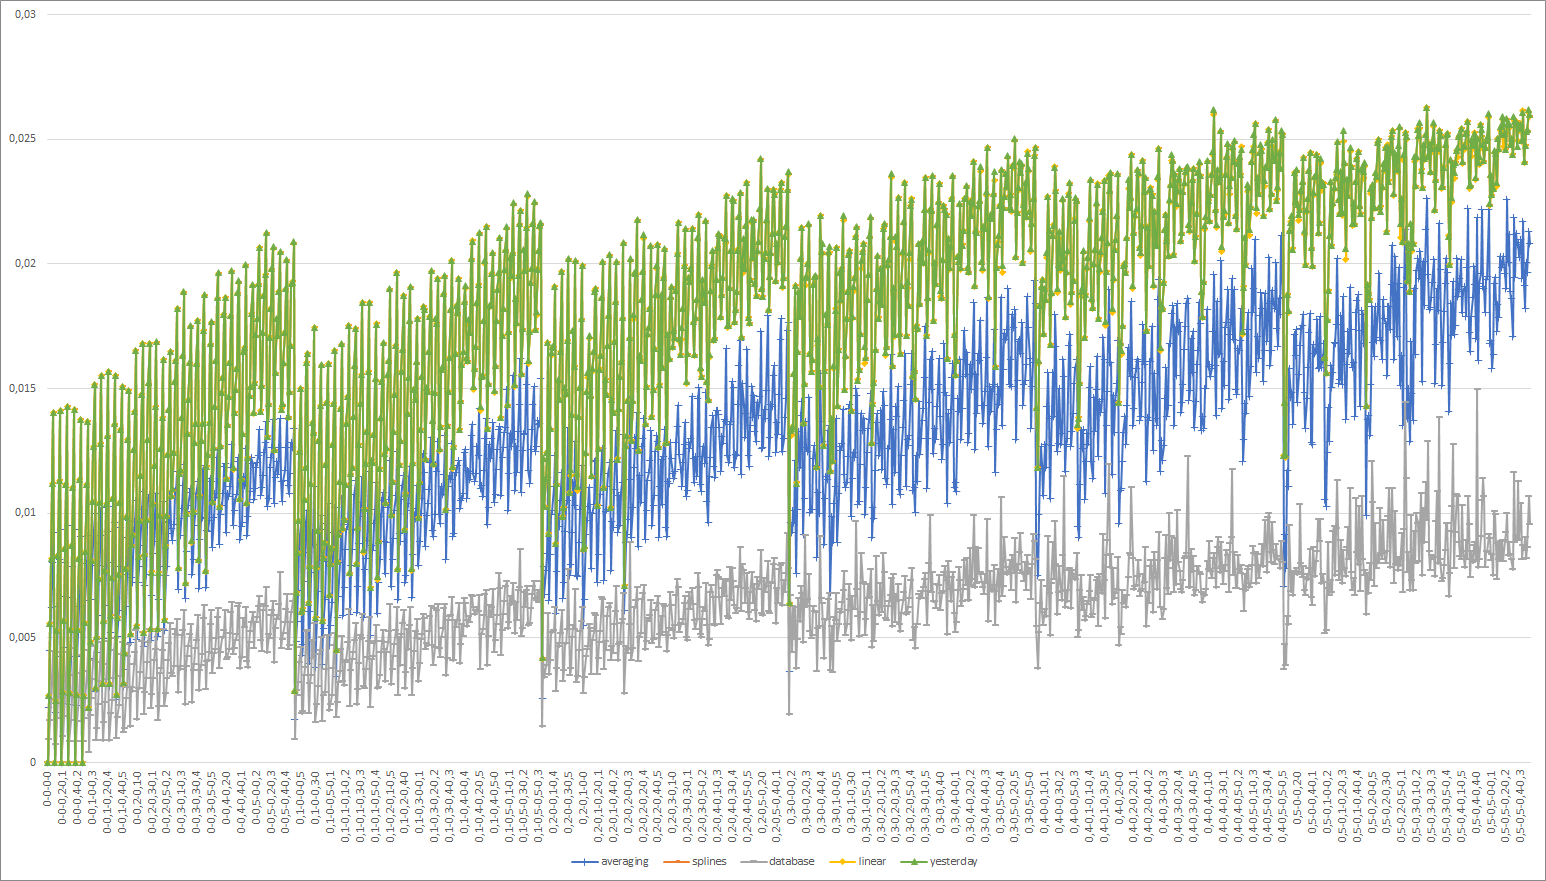
\includegraphics[width=0.9\columnwidth]{pics/evaluation-algorithms}
	\end{center}
	\caption{\label{fig:evaluation_algorithms}Gesamtergebnisse ohne Newton}
\end{figure}

Zunächst fällt bei der Betrachtung der Ergebnisse auf, dass der Newton-Ansatz bei kleinen Lücken sehr gute Ergebnisse liefert, während sehr große Lücken in überaus hohen Distanzwerten resultieren. Dies liegt an der gebildeten Polynomfunktion, deren Werte bei großen Lücken stark nach oben oder unten ausreißen können.
Die Bewertungen der anderen Algorithmen finden sich alle in einem vergleichsweise geringen Bereich wieder, wie in Abbildung~\ref{fig:evaluation_algorithms} zu erkennen ist. Je mehr Daten fehlen, desto großer ist der Fehlerwert. Dies gilt für alle Algorithmen. Die Werte innerhalb der Abbildung springen, da vier verschiedene Konfigurationsparameter auf eine Dimension reduziert werden mussten. Die fünf gleichmäßig verteilten Sprünge markieren die Stellen, an denen der Anteil entfernter Wochen zurückgesetzt wurde. Daraus resultierend sinkt der Anteil insgesamt entfernter Messwerte.
Der Test liefert sehr ähnliche Werte für die lineare Interpolation (In der Abbildung gelb), sowie für die Interpolation basierend auf Splines (Orange) und den Daten des Vortages (Grün). Ein besseres Ergebnis liefert die Mittelwertinterpolation (Blau). Innerhalb der sehr künstlichen Bedingungen liefert der Datenbankansatz (graue Linie) das beste Ergebnis.

\begin{figure}[!t]
	\begin{center}
		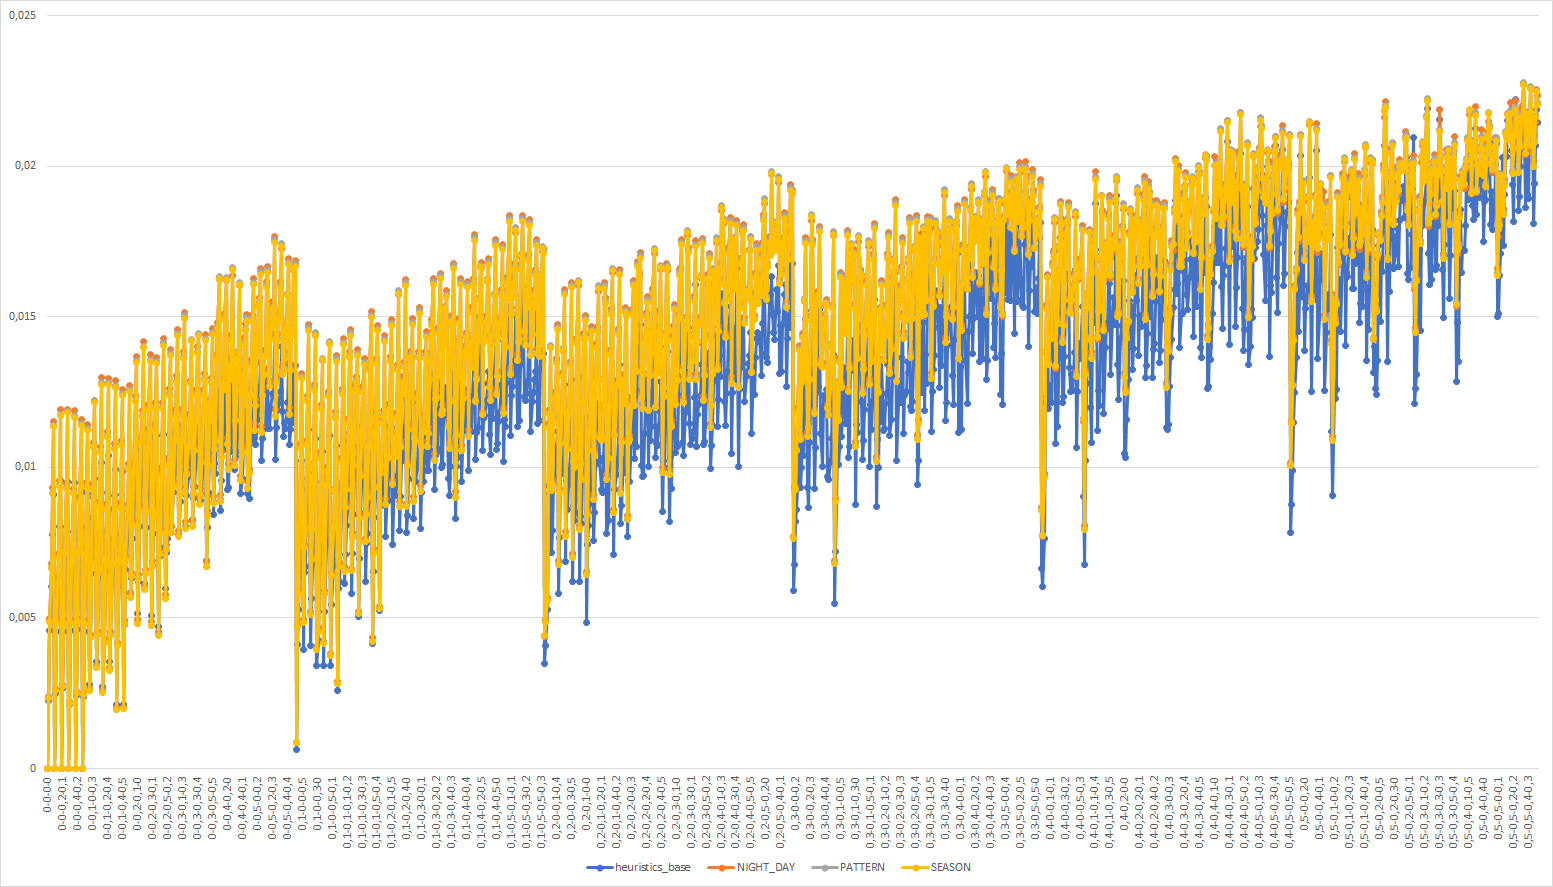
\includegraphics[width=0.9\columnwidth]{pics/evaluation-heuristics}
	\end{center}
	\caption{\label{fig:evaluation_heuristics}Gesamtergebnisse der Heuristiken}
\end{figure}

Als Basis für die Bewertung der Heuristiken dient ein mithilfe des Mittelwertverfahrens interpolierter Lastgang ebenfalls mit derselben Variation in den zufällig eingefügten Lücken. Wie in Abbildung~\ref{fig:evaluation_heuristics} zu erkennen lässt sich ein ähnlicher Grundtrend wie bei den Algorithmen beobachten. Mit steigender Anzahl an Lücken nimmt der Distanzwert ebenfalls zu. Die drei Heuristiken produzieren sehr ähnliche Ergebnisse, die in diesem Test leicht über den Werten der lediglich mit der Durchschnittsbildung interpolierten Basis liegen.
Die Verschlechterung ist zu beobachten, da die Ergebnisse der Mittelwertbildung ohne nachfolgende Interpolation ohnehin bereits sehr gut sind. In Verbindung mit anderen, schlechteren Interpolationsverfahren verbessern die Heuristiken die Ergebnisse. Dies gilt insbesondere für das Newton-Verfahren, dessen Bewertung sehr schlecht für größere Lücken ist. Mit nachfolgender Anwendung einer Heuristik verschiebt sich die Bewertung des Newton-Verfahren in die Nähe der anderen Interpolationsverfahren.
Somit dienen die umgesetzten Heuristiken nicht der allgemeinen Verbesserung, sondern helfen bei der Validierung und daraus resultierenden Anpassung von Ausreißern, wie bei Newton beobachtet.